% ============================================================
% Cylindrical Void in a Rigid-Ideally Plastic BCC Single Crystal
% Target: International Journal of Plasticity (IJP) or
%         Journal of the Mechanics and Physics of Solids (JMPS)
% ============================================================
\documentclass[smallextended,natbib]{svjour3}
\smartqed
\usepackage{amsmath,amssymb,bm}
\usepackage{graphicx}
\usepackage{booktabs}
\usepackage{multirow}
\usepackage{xcolor}
\usepackage{tikz}

% Journal name
\journalname{International Journal of Plasticity}

% Short-hand macros
\newcommand{\bsig}{\bm{\sigma}}
\newcommand{\btau}{\bm{\tau}}
\newcommand{\bn}{\hat{\mathbf{n}}}
\newcommand{\bs}{\hat{\mathbf{s}}}
\newcommand{\bP}{\mathbf{P}}
\newcommand{\bF}{\mathbf{F}}
\newcommand{\bI}{\mathbf{I}}
\newcommand{\bR}{\mathbf{R}}
\newcommand{\be}{\mathbf{e}}
\newcommand{\bx}{\mathbf{x}}
\newcommand{\diff}{\mathrm{d}}
\newcommand{\abs}[1]{\lvert #1 \rvert}
\newcommand{\tcrss}{\tau_{\mathrm{CRSS}}}
\newcommand{\srr}{\sigma_{rr}}
\newcommand{\stt}{\sigma_{\theta\theta}}
\newcommand{\srt}{\sigma_{r\theta}}
\newcommand{\sm}{\sigma_m}

\begin{document}

\title{Cylindrical void in a rigid-ideally plastic single crystal.
Part~IV: Body-centered cubic crystal}

\author{WaiChing Sun}

\institute{
W.~Sun \at
Department of Civil Engineering and Engineering Mechanics,
Columbia University, New York, NY 10027, USA \\
\email{ws2407@columbia.edu}
}

\date{Received: date / Accepted: date}

\maketitle

% ============================================================
\begin{abstract}
Anisotropic slip line theory is employed to derive the stress and deformation
state around a cylindrical void in a body-centered cubic (BCC) single crystal
oriented so that plane strain conditions are admitted from the
$\{110\}\langle 111\rangle$ slip system family. The void axis is parallel to
the $[110]$ crystallographic direction, which reduces the twelve
three-dimensional slip systems to three distinct effective in-plane yield
constraints. A hexagonal yield polygon is constructed in the Mohr stress
plane. The polygon is elongated relative to the face-centered cubic (FCC)
case, with an aspect ratio of $\sqrt{8/3} \approx 1.63$ compared to
$\sqrt{2/3} \approx 0.82$ for FCC. The stress field around the void is
decomposed into six angular sectors in $[0, \pi]$ with exact boundaries
at $\theta_1 = \frac{1}{2}\arctan(2\sqrt{2})$ and
$\theta_2 = \frac{1}{2}[\pi - \arctan(2\sqrt{2})]$.
The activation pressure for plastic flow around the void is found to be
$p^* = \frac{3\sqrt{6}}{4}\,\tcrss \approx 1.84\,\tcrss$, which is 50\%
higher than the FCC result of
$p^*_{\mathrm{FCC}} = \frac{\sqrt{6}}{2}\,\tcrss \approx 1.22\,\tcrss$.
This provides a quantitative, single-crystal-level explanation for the
well-documented superior resistance of BCC metals to radiation-induced
void swelling compared to FCC metals. The plastic zone surrounding the void
is predicted to be non-circular, with a four-lobed shape reflecting the
crystal symmetry of the $(110)$ plane.

\keywords{
Crystal plasticity \and
Slip line theory \and
Void growth \and
BCC single crystal \and
Ductile fracture \and
Radiation damage
}
\end{abstract}

% ============================================================
\section{Introduction}
\label{sec:intro}
% ============================================================

Ductile fracture in metals is governed by the nucleation, growth, and
coalescence of microscale voids. The seminal analytical treatments of void
growth~\citep{mcclintock1968,rice1969} assumed an isotropic material
surrounding the void. However, at the scale of individual voids, the
surrounding material is a single crystal with strongly anisotropic plastic
response. Understanding the single-crystal stress and deformation fields
around voids is essential for physics-based ductile fracture models.

\citet{rice1973} developed the anisotropic slip line theory for
rigid-ideally plastic materials under plane strain, generalizing the
classical Hencky equations to materials with arbitrary in-plane yield
contour. This framework was applied by \citet{rice1987} to derive the
asymptotic crack-tip stress fields in FCC and BCC single crystals.
\citet{drugan2001} extended these crack-tip solutions to include elastic
sectors, demonstrating that FCC and BCC crystals produce distinct
crack-tip fields.

\citet{kysar2005} (hereafter referred to as Part~I) applied Rice's
anisotropic slip line theory to derive the complete stress field around a
cylindrical void in an FCC single crystal. The void axis was aligned with
$[110]$, reducing the twelve $\{111\}\langle 110\rangle$ slip systems to
three effective in-plane systems. The resulting hexagonal yield polygon
and sector-based stress field provided the first analytical benchmark for
void growth in anisotropic single crystals. \citet{gan2006} (Part~II)
validated the analytical solution against experiments on copper single
crystals and crystal plasticity finite element (CPFE) simulations.
\citet{gan2007} (Part~III) extended the analysis to hexagonal close-packed
(HCP) crystals.

Despite the practical importance of BCC metals --- iron, tungsten,
molybdenum, and their alloys form the backbone of structural engineering
--- no analytical solution exists for the void problem in a BCC single
crystal. This gap is particularly notable given that BCC
ferritic/martensitic steels exhibit significantly superior resistance to
radiation-induced void swelling compared to FCC austenitic
steels~\citep{garner2010,zinkle2013}. A quantitative, single-crystal-level
understanding of this difference has been lacking.

The present work fills this gap by deriving the analytical stress field
around a cylindrical void in a rigid-ideally plastic BCC single crystal
with $\{110\}\langle 111\rangle$ slip, constituting Part~IV of the Kysar
series. The analysis reveals that: (i)~the BCC yield polygon is an
elongated hexagon rotated by $\arctan(2\sqrt{2})/2 \approx 35.3^\circ$
relative to FCC; (ii)~the activation pressure for void growth is exactly
50\% higher than FCC; and (iii)~the plastic zone around the void is
non-circular, with a four-lobed shape reflecting the crystal symmetry.

The remainder of this paper is organized as follows.
Section~\ref{sec:crystal} defines the BCC crystal geometry and derives
the effective in-plane slip systems.
Section~\ref{sec:yield} constructs the yield polygon.
Section~\ref{sec:stress} derives the sector-based stress field.
Section~\ref{sec:interior} extends the solution to the interior.
Section~\ref{sec:comparison} compares BCC and FCC results.
Section~\ref{sec:numerical} presents numerical verification.
Section~\ref{sec:discussion} discusses physical implications.
Section~\ref{sec:conclusions} concludes.

% ============================================================
\section{Crystal geometry and effective slip systems}
\label{sec:crystal}
% ============================================================

\subsection{BCC $\{110\}\langle 111\rangle$ slip systems}

The body-centered cubic lattice admits slip on the $\{110\}$ family of
planes in the $\langle 111\rangle$ family of directions. This gives twelve
slip systems $\alpha = 1, \ldots, 12$, each defined by a slip plane normal
$\bn^\alpha$ and a slip direction $\bs^\alpha$ (Table~\ref{tab:slip}).

\begin{table}[htb]
\caption{The twelve BCC $\{110\}\langle 111\rangle$ slip systems.}
\label{tab:slip}
\centering
\begin{tabular}{ccc|ccc}
\toprule
$\alpha$ & Plane $(hkl)$ & Direction $[uvw]$ &
$\alpha$ & Plane $(hkl)$ & Direction $[uvw]$ \\
\midrule
1  & $(110)$         & $[\bar{1}11]$        & 7  & $(10\bar{1})$   & $[111]$ \\
2  & $(110)$         & $[1\bar{1}1]$        & 8  & $(10\bar{1})$   & $[\bar{1}1\bar{1}]$ \\
3  & $(1\bar{1}0)$   & $[111]$              & 9  & $(011)$         & $[1\bar{1}1]$ \\
4  & $(1\bar{1}0)$   & $[\bar{1}\bar{1}1]$  & 10 & $(011)$         & $[11\bar{1}]$ \\
5  & $(101)$         & $[\bar{1}11]$        & 11 & $(01\bar{1})$   & $[111]$ \\
6  & $(101)$         & $[11\bar{1}]$        & 12 & $(01\bar{1})$   & $[1\bar{1}\bar{1}]$ \\
\bottomrule
\end{tabular}
\end{table}

The resolved shear stress on system $\alpha$ is
$\tau^\alpha = P^\alpha_{ij}\,\sigma_{ij}$, where the Schmid tensor is
\begin{equation}
\label{eq:schmid}
P^\alpha_{ij} = \tfrac{1}{2}(\hat{s}^\alpha_i \hat{n}^\alpha_j
                            + \hat{s}^\alpha_j \hat{n}^\alpha_i).
\end{equation}
Plastic flow on system $\alpha$ occurs when
$|\tau^\alpha| = \tcrss$, where $\tcrss$ is the critical resolved shear
stress, assumed equal on all systems.

\subsection{Plane strain coordinate system}

We consider a cylindrical void with axis parallel to $[110]$. The plane
strain coordinate system is defined by (Fig.~\ref{fig:geometry}):
\begin{equation}
\label{eq:coords}
\be'_1 = [001], \qquad
\be'_2 = \frac{1}{\sqrt{2}}[\bar{1}10], \qquad
\be'_3 = \frac{1}{\sqrt{2}}[110].
\end{equation}
The rotation from crystal to primed coordinates is
\begin{equation}
\label{eq:rotation}
\bR = \begin{pmatrix}
0 & 0 & 1 \\
-1/\sqrt{2} & 1/\sqrt{2} & 0 \\
1/\sqrt{2} & 1/\sqrt{2} & 0
\end{pmatrix}.
\end{equation}

\begin{figure}[htb]
\centering
% TODO: Insert geometry schematic
% \includegraphics[width=0.6\textwidth]{fig_geometry}
\caption{Problem geometry: cylindrical void of radius $a$ in a BCC single
crystal with void axis along $[110]$. The in-plane coordinate system is
$\be'_1 = [001]$, $\be'_2 = [\bar{1}10]/\sqrt{2}$.}
\label{fig:geometry}
\end{figure}

\subsection{Effective in-plane systems}
\label{sec:effective}

Transforming all twelve Schmid tensors to primed coordinates and computing
the in-plane resolved shear stress
$\tau^\alpha = a^\alpha X + b^\alpha Y$, where
$X = (\sigma_{11} - \sigma_{22})/2$ and $Y = \sigma_{12}$ are the Mohr
plane coordinates, yields the results in Table~\ref{tab:schmid2d}.

\begin{table}[htb]
\caption{In-plane Schmid coefficients $a^\alpha$, $b^\alpha$ such that
$\tau^\alpha = a^\alpha X + b^\alpha Y$.}
\label{tab:schmid2d}
\centering
\begin{tabular}{ccc|ccc}
\toprule
$\alpha$ & $a^\alpha$ & $b^\alpha$ &
$\alpha$ & $a^\alpha$ & $b^\alpha$ \\
\midrule
1, 2  & $0$ & $0$ &
7, 10 & $-\sqrt{6}/3$ & $-\sqrt{3}/6$ \\
3, 4  & $0$ & $-\sqrt{3}/3$ &
8, 9  & $+\sqrt{6}/3$ & $-\sqrt{3}/6$ \\
5, 12 & $+\sqrt{6}/3$ & $+\sqrt{3}/6$ &
6, 11 & $-\sqrt{6}/3$ & $+\sqrt{3}/6$ \\
\bottomrule
\end{tabular}
\end{table}

A key finding is that systems 1 and 2, which lie on the $(110)$ plane
containing the void axis, have \emph{identically zero} in-plane Schmid
tensor components. These systems contribute only anti-plane shear
deformation and do not participate in the plane strain yield surface. This
is a structural consequence of the $(110)$ plane being perpendicular to the
deformation plane.

The ten active systems (3--12) produce three \emph{distinct} yield
constraints:
\begin{align}
\label{eq:yield_constraints}
\text{(I)} & \quad
  \left\lvert -\frac{\sqrt{3}}{3}\,Y \right\rvert \leq \tcrss
  & & \text{(systems 3, 4)}, \\
\text{(II)} & \quad
  \left\lvert \frac{\sqrt{6}}{3}\,X
            + \frac{\sqrt{3}}{6}\,Y \right\rvert \leq \tcrss
  & & \text{(systems 5, 12)}, \\
\text{(III)} & \quad
  \left\lvert -\frac{\sqrt{6}}{3}\,X
             + \frac{\sqrt{3}}{6}\,Y \right\rvert \leq \tcrss
  & & \text{(systems 6, 11)}.
\end{align}

For plane strain, individual 3D systems combine pairwise to eliminate
out-of-plane strain components ($d_{33} = d_{13} = d_{23} = 0$). Systems
3 and 4 form a same-plane pair on $(1\bar{1}0)$. The remaining pairs
(e.g., 5+12, 8+9) involve cross-plane combinations --- a structural
difference from FCC, where all effective pairs are same-plane.

% ============================================================
\section{Yield polygon in the Mohr stress plane}
\label{sec:yield}
% ============================================================

The three yield constraints~\eqref{eq:yield_constraints}, each defining
a pair of parallel lines in the $(X, Y)$ Mohr stress plane, intersect to
form a hexagonal yield polygon (Fig.~\ref{fig:yield_surface}).

\subsection{Vertices}

The six vertices, in units of $\tcrss$, are:
\begin{equation}
\label{eq:vertices}
\begin{aligned}
V_1 &= \bigl(-\tfrac{\sqrt{6}}{4},\; -\sqrt{3}\bigr), &
V_2 &= \bigl(+\tfrac{\sqrt{6}}{4},\; -\sqrt{3}\bigr), &
V_3 &= \bigl(+\tfrac{\sqrt{6}}{2},\; 0\bigr), \\
V_4 &= \bigl(+\tfrac{\sqrt{6}}{4},\; +\sqrt{3}\bigr), &
V_5 &= \bigl(-\tfrac{\sqrt{6}}{4},\; +\sqrt{3}\bigr), &
V_6 &= \bigl(-\tfrac{\sqrt{6}}{2},\; 0\bigr).
\end{aligned}
\end{equation}
The polygon has half-width $|X|_{\max} = \sqrt{6}/2 \approx 1.225\,\tcrss$
and half-height $|Y|_{\max} = \sqrt{3} \approx 1.732\,\tcrss$, giving an
aspect ratio (height/width) of $\sqrt{8/3} \approx 1.633$.

\subsection{Faces}

\begin{table}[htb]
\caption{Yield polygon faces and active slip systems.}
\label{tab:faces}
\centering
\begin{tabular}{lll}
\toprule
Face & Equation & Active systems \\
\midrule
$V_1 \to V_2$ & $Y = -\sqrt{3}$  & 3, 4 \\
$V_2 \to V_3$ & $\frac{\sqrt{6}}{3}X - \frac{\sqrt{3}}{6}Y = 1$ & 8, 9 \\
$V_3 \to V_4$ & $\frac{\sqrt{6}}{3}X + \frac{\sqrt{3}}{6}Y = 1$ & 5, 12 \\
$V_4 \to V_5$ & $Y = +\sqrt{3}$  & 3, 4 \\
$V_5 \to V_6$ & $-\frac{\sqrt{6}}{3}X - \frac{\sqrt{3}}{6}Y = 1$ & 7, 10 \\
$V_6 \to V_1$ & $-\frac{\sqrt{6}}{3}X + \frac{\sqrt{3}}{6}Y = -1$ & 6, 11 \\
\bottomrule
\end{tabular}
\end{table}

\begin{figure}[htb]
\centering
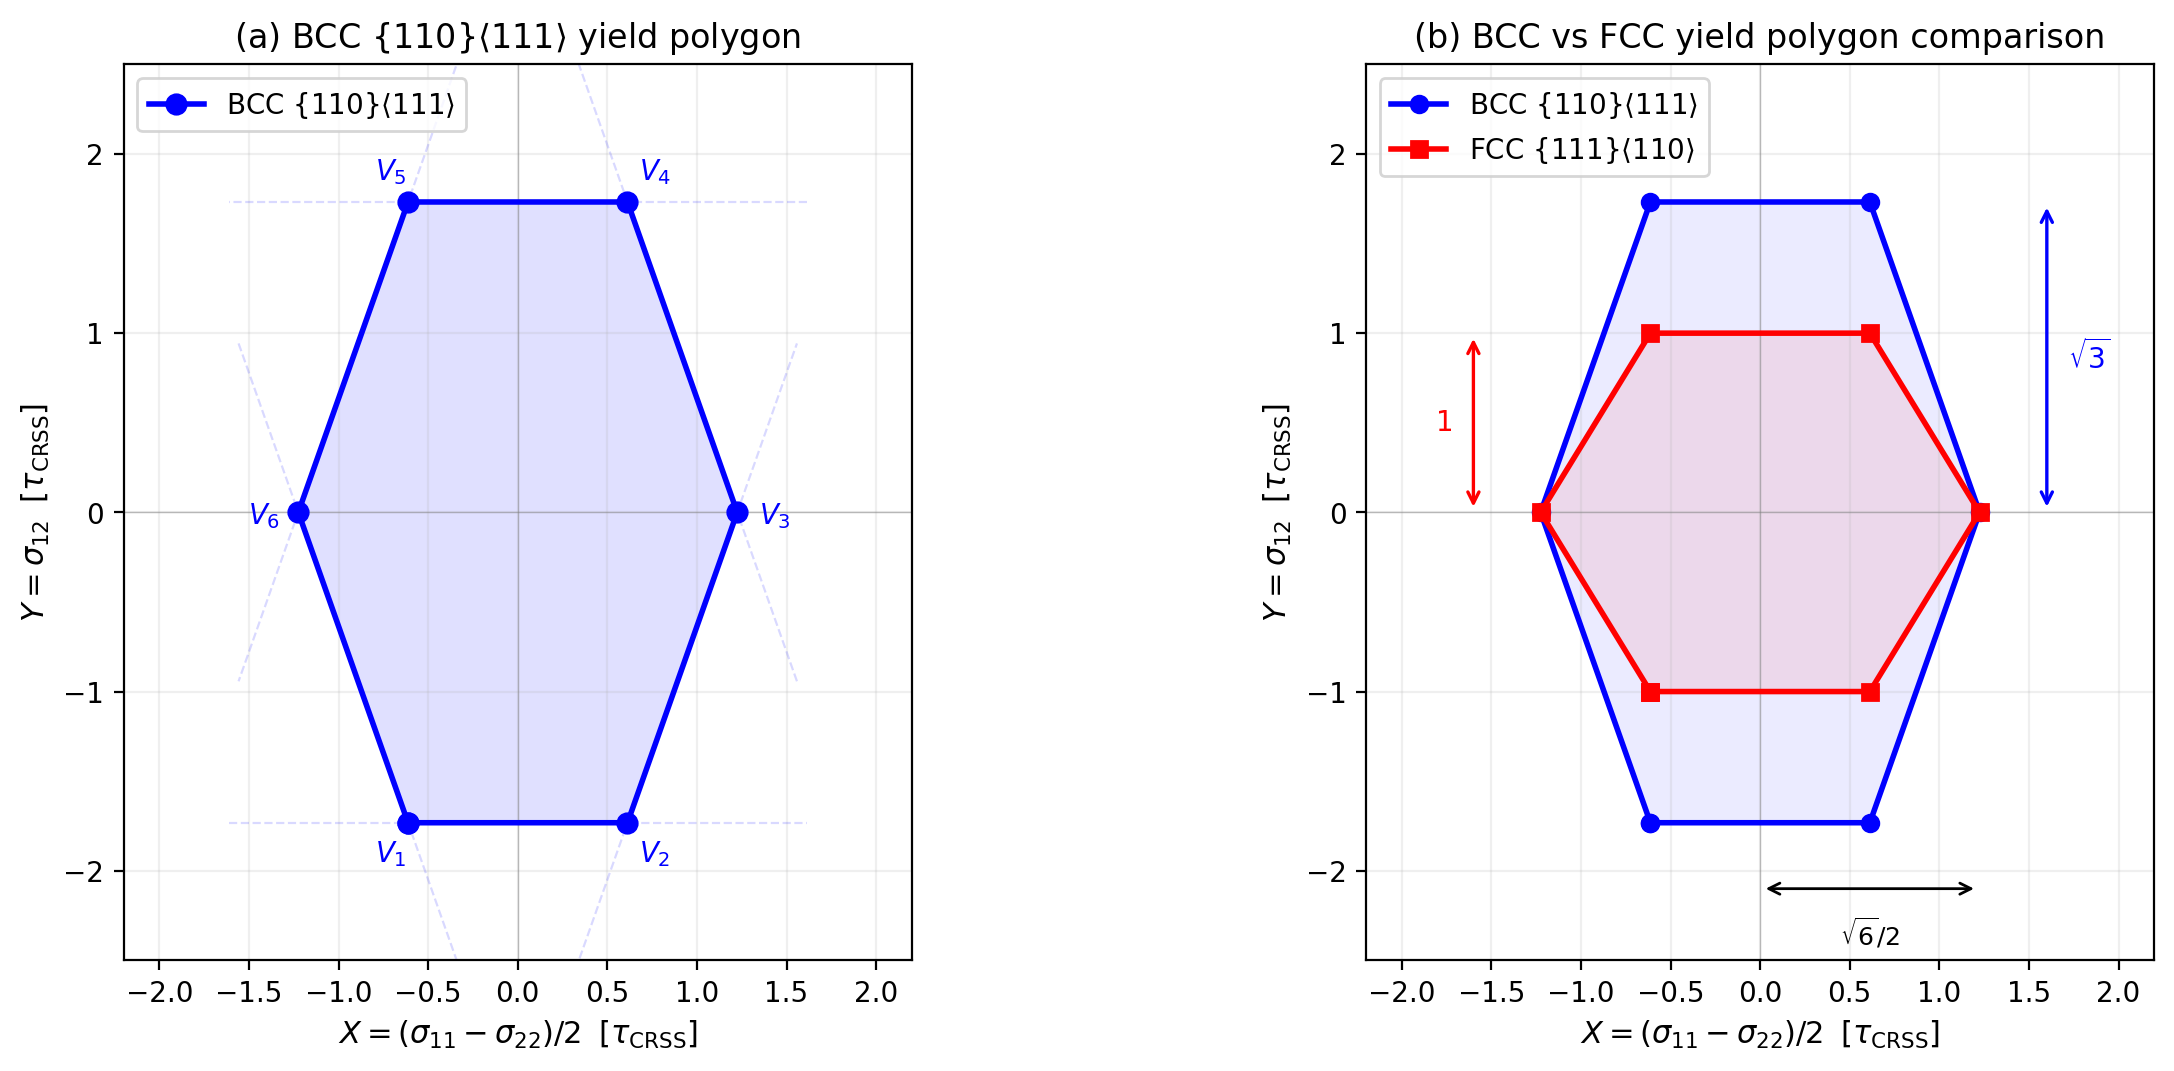
\includegraphics[width=0.95\textwidth]{../figures/bcc_vs_fcc_yield_surface}
\caption{(a)~BCC $\{110\}\langle 111\rangle$ yield polygon in the Mohr
stress plane. (b)~Comparison of BCC (blue) and FCC
$\{111\}\langle 110\rangle$ (red) yield polygons. Both are hexagons; the
BCC polygon is elongated in the $Y$ direction and rotated by
$\arctan(2\sqrt{2})/2 \approx 35.3^\circ$.}
\label{fig:yield_surface}
\end{figure}

% ============================================================
\section{Stress field around the void}
\label{sec:stress}
% ============================================================

\subsection{Problem statement}

Consider a cylindrical void of radius $a$ in an infinite rigid-ideally
plastic BCC single crystal under equibiaxial far-field compression
$\sigma_{rr} = \stt = -p$ at $r \to \infty$.
The void surface ($r = a$) is traction-free:
\begin{equation}
\label{eq:bc_void}
\srr(a, \theta) = 0, \qquad \srt(a, \theta) = 0.
\end{equation}

\subsection{Rice's anisotropic slip line theory}

Following \citet{rice1973}, the stress field in the fully plastic region
satisfies two equilibrium equations in polar coordinates:
\begin{align}
\label{eq:equil1}
\frac{\partial \srr}{\partial r}
  + \frac{\srr - \stt}{r}
  + \frac{1}{r}\frac{\partial \srt}{\partial \theta} &= 0, \\
\label{eq:equil2}
\frac{\partial \srt}{\partial r}
  + \frac{2\srt}{r}
  + \frac{1}{r}\frac{\partial \stt}{\partial \theta} &= 0.
\end{align}
The polar and Cartesian stress components are related by
\begin{align}
\label{eq:polar_cart}
\srr &= \sm + X\cos 2\theta + Y\sin 2\theta, \\
\stt &= \sm - X\cos 2\theta - Y\sin 2\theta, \\
\srt &= -X\sin 2\theta + Y\cos 2\theta,
\end{align}
where $\sm = (\sigma_{11} + \sigma_{22})/2$ is the mean in-plane stress.

The generalized Hencky equations~\citep{rice1973} state that along the
two families of characteristics (slip lines):
\begin{equation}
\label{eq:hencky}
\sm + s = \text{const along } \alpha\text{-lines}, \qquad
\sm - s = \text{const along } \beta\text{-lines},
\end{equation}
where $s$ is the arc length along the yield contour in the Mohr stress
plane.

\subsection{Void surface stress}

The traction-free conditions~\eqref{eq:bc_void} require
\begin{equation}
\label{eq:void_constraint}
Y = X\tan 2\theta, \qquad
\sm = -\frac{X}{\cos 2\theta}.
\end{equation}
Combined with the active yield face equation $aX + bY = \pm\tcrss$,
this gives the deviatoric stress at the void surface as
\begin{equation}
\label{eq:X_void}
X(\theta) = \frac{\pm\tcrss}{a + b\tan 2\theta}.
\end{equation}

\subsection{Sector structure}
\label{sec:sectors}

The sector boundaries occur at angles where the void surface stress
passes through a vertex of the yield polygon. Since each vertex lies at
Mohr angle $\alpha_V$, the corresponding physical angle is
$\theta = \alpha_V / 2$. The key angle is
\begin{equation}
\label{eq:key_angle}
\arctan(2\sqrt{2}) \approx 70.53^\circ,
\end{equation}
which gives the sector boundaries listed in Table~\ref{tab:sectors}.

\begin{table}[htb]
\caption{Sector structure: angular regions and active yield faces.}
\label{tab:sectors}
\centering
\begin{tabular}{clll}
\toprule
Sector & $\theta$ range & Active face & Systems \\
\midrule
I   & $0 < \theta < \theta_1$ & $V_3 \to V_4$ & 5, 12 \\
II  & $\theta_1 < \theta < \theta_2$ & $V_4 \to V_5$ & 3, 4 \\
III & $\theta_2 < \theta < \pi/2$ & $V_5 \to V_6$ & 6, 11 \\
IV  & $\pi/2 < \theta < \pi - \theta_2$ & mirror of III & 5, 12 \\
V   & $\pi - \theta_2 < \theta < \pi - \theta_1$ & mirror of II & 3, 4 \\
VI  & $\pi - \theta_1 < \theta < \pi$ & mirror of I & 6, 11 \\
\bottomrule
\end{tabular}\\[4pt]
\footnotesize
$\theta_1 = \frac{1}{2}\arctan(2\sqrt{2}) \approx 35.26^\circ$, \quad
$\theta_2 = \frac{1}{2}[\pi - \arctan(2\sqrt{2})] \approx 54.74^\circ$.
\end{table}

\subsection{Exact void surface stress in each sector}

\paragraph{Sector~I} ($0 < \theta < \theta_1$; face $V_3 \to V_4$,
$\frac{\sqrt{6}}{3}X + \frac{\sqrt{3}}{6}Y = \tcrss$):
\begin{equation}
\label{eq:sector1}
\sm(\theta) = \frac{-6\,\tcrss}
  {\sqrt{3}\sin 2\theta + 2\sqrt{6}\cos 2\theta}, \qquad
\stt(\theta) = 2\,\sm(\theta).
\end{equation}

\paragraph{Sector~II} ($\theta_1 < \theta < \theta_2$; face $V_4 \to V_5$,
$Y = \sqrt{3}\,\tcrss$):
\begin{equation}
\label{eq:sector2}
\sm(\theta) = \frac{-\sqrt{3}\,\tcrss}{\sin 2\theta}, \qquad
\stt(\theta) = 2\,\sm(\theta), \qquad
\sigma_{12} = \sqrt{3}\,\tcrss \;\text{(constant)}.
\end{equation}

\paragraph{Sector~III} ($\theta_2 < \theta < \pi/2$; face $V_5 \to V_6$,
$-\frac{\sqrt{6}}{3}X + \frac{\sqrt{3}}{6}Y = -\tcrss$):
\begin{equation}
\label{eq:sector3}
\sm(\theta) = \frac{6\,\tcrss}
  {\sqrt{3}\sin 2\theta - 2\sqrt{6}\cos 2\theta}, \qquad
\stt(\theta) = 2\,\sm(\theta).
\end{equation}
Sectors IV--VI follow by mirror symmetry about $\theta = \pi/2$.

\begin{figure}[htb]
\centering
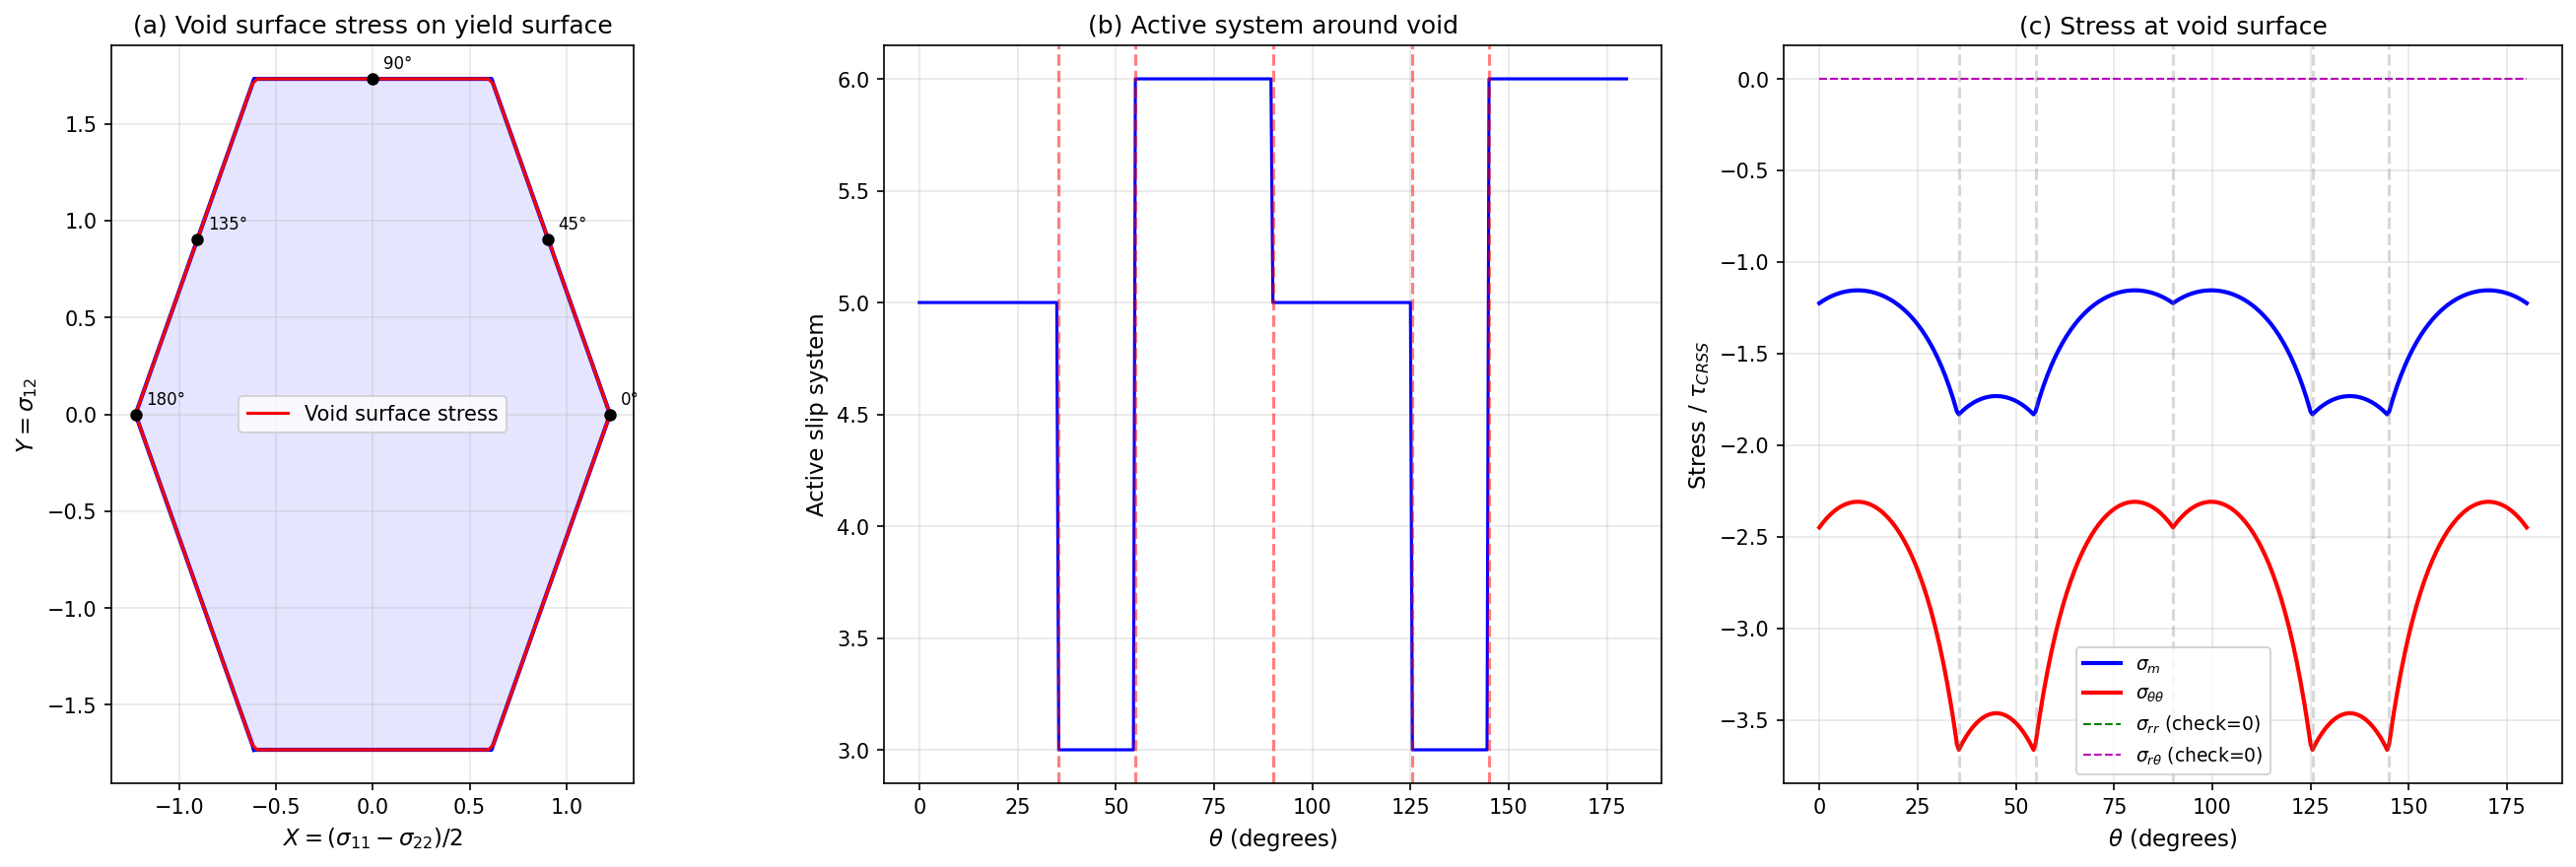
\includegraphics[width=0.95\textwidth]{../figures/sector_structure}
\caption{(a)~Void surface stress path on the BCC yield polygon.
(b)~Active slip system versus angle $\theta$.
(c)~Stress components $\sm$ and $\stt$ at the void surface.}
\label{fig:sector_structure}
\end{figure}

% ============================================================
\section{Interior stress field and plastic zone}
\label{sec:interior}
% ============================================================

\subsection{Radial stress variation}

Within the plastic zone ($a \leq r \leq R(\theta)$), the stress satisfies
equilibrium and the yield condition simultaneously. The leading-order
solution, which generalizes the classical isotropic result
$\srr = -2k\ln(r/a)$, is:
\begin{align}
\label{eq:interior}
\srr(r, \theta) &= \stt(a, \theta) \cdot \ln(r/a), \\
\stt(r, \theta) &= \stt(a, \theta) \cdot [1 + \ln(r/a)], \\
\sm(r, \theta)  &= \stt(a, \theta) \cdot [\tfrac{1}{2} + \ln(r/a)],
\end{align}
where $\stt(a, \theta)$ is the exact hoop stress at the void surface
given by~\eqref{eq:sector1}--\eqref{eq:sector3}. The angle-dependent
coefficient $\stt(a, \theta)$ encodes the crystal anisotropy, replacing
the constant $-2k$ of the isotropic solution.

\subsection{Non-circular plastic zone}

The far-field condition $\srr(R, \theta) = -p$ determines the plastic
zone boundary:
\begin{equation}
\label{eq:plastic_zone}
\frac{R(\theta)}{a}
  = \exp\!\left(\frac{p}{\abs{\stt(a, \theta)}}\right).
\end{equation}
Since $\abs{\stt(a, \theta)}$ varies with $\theta$ --- from a minimum of
$\sqrt{6}\,\tcrss$ at $\theta = 0^\circ$ and $90^\circ$ to a maximum of
$\frac{3\sqrt{6}}{2}\,\tcrss$ at the sector boundaries --- the plastic
zone is \emph{non-circular} (Fig.~\ref{fig:interior}). The zone is
elongated along the $\be'_1 = [001]$ and $\be'_2 = [\bar{1}10]/\sqrt{2}$
directions and compressed at the sector boundaries, producing a
four-lobed shape that reflects the crystal symmetry of the $(110)$ plane.

\begin{figure}[htb]
\centering
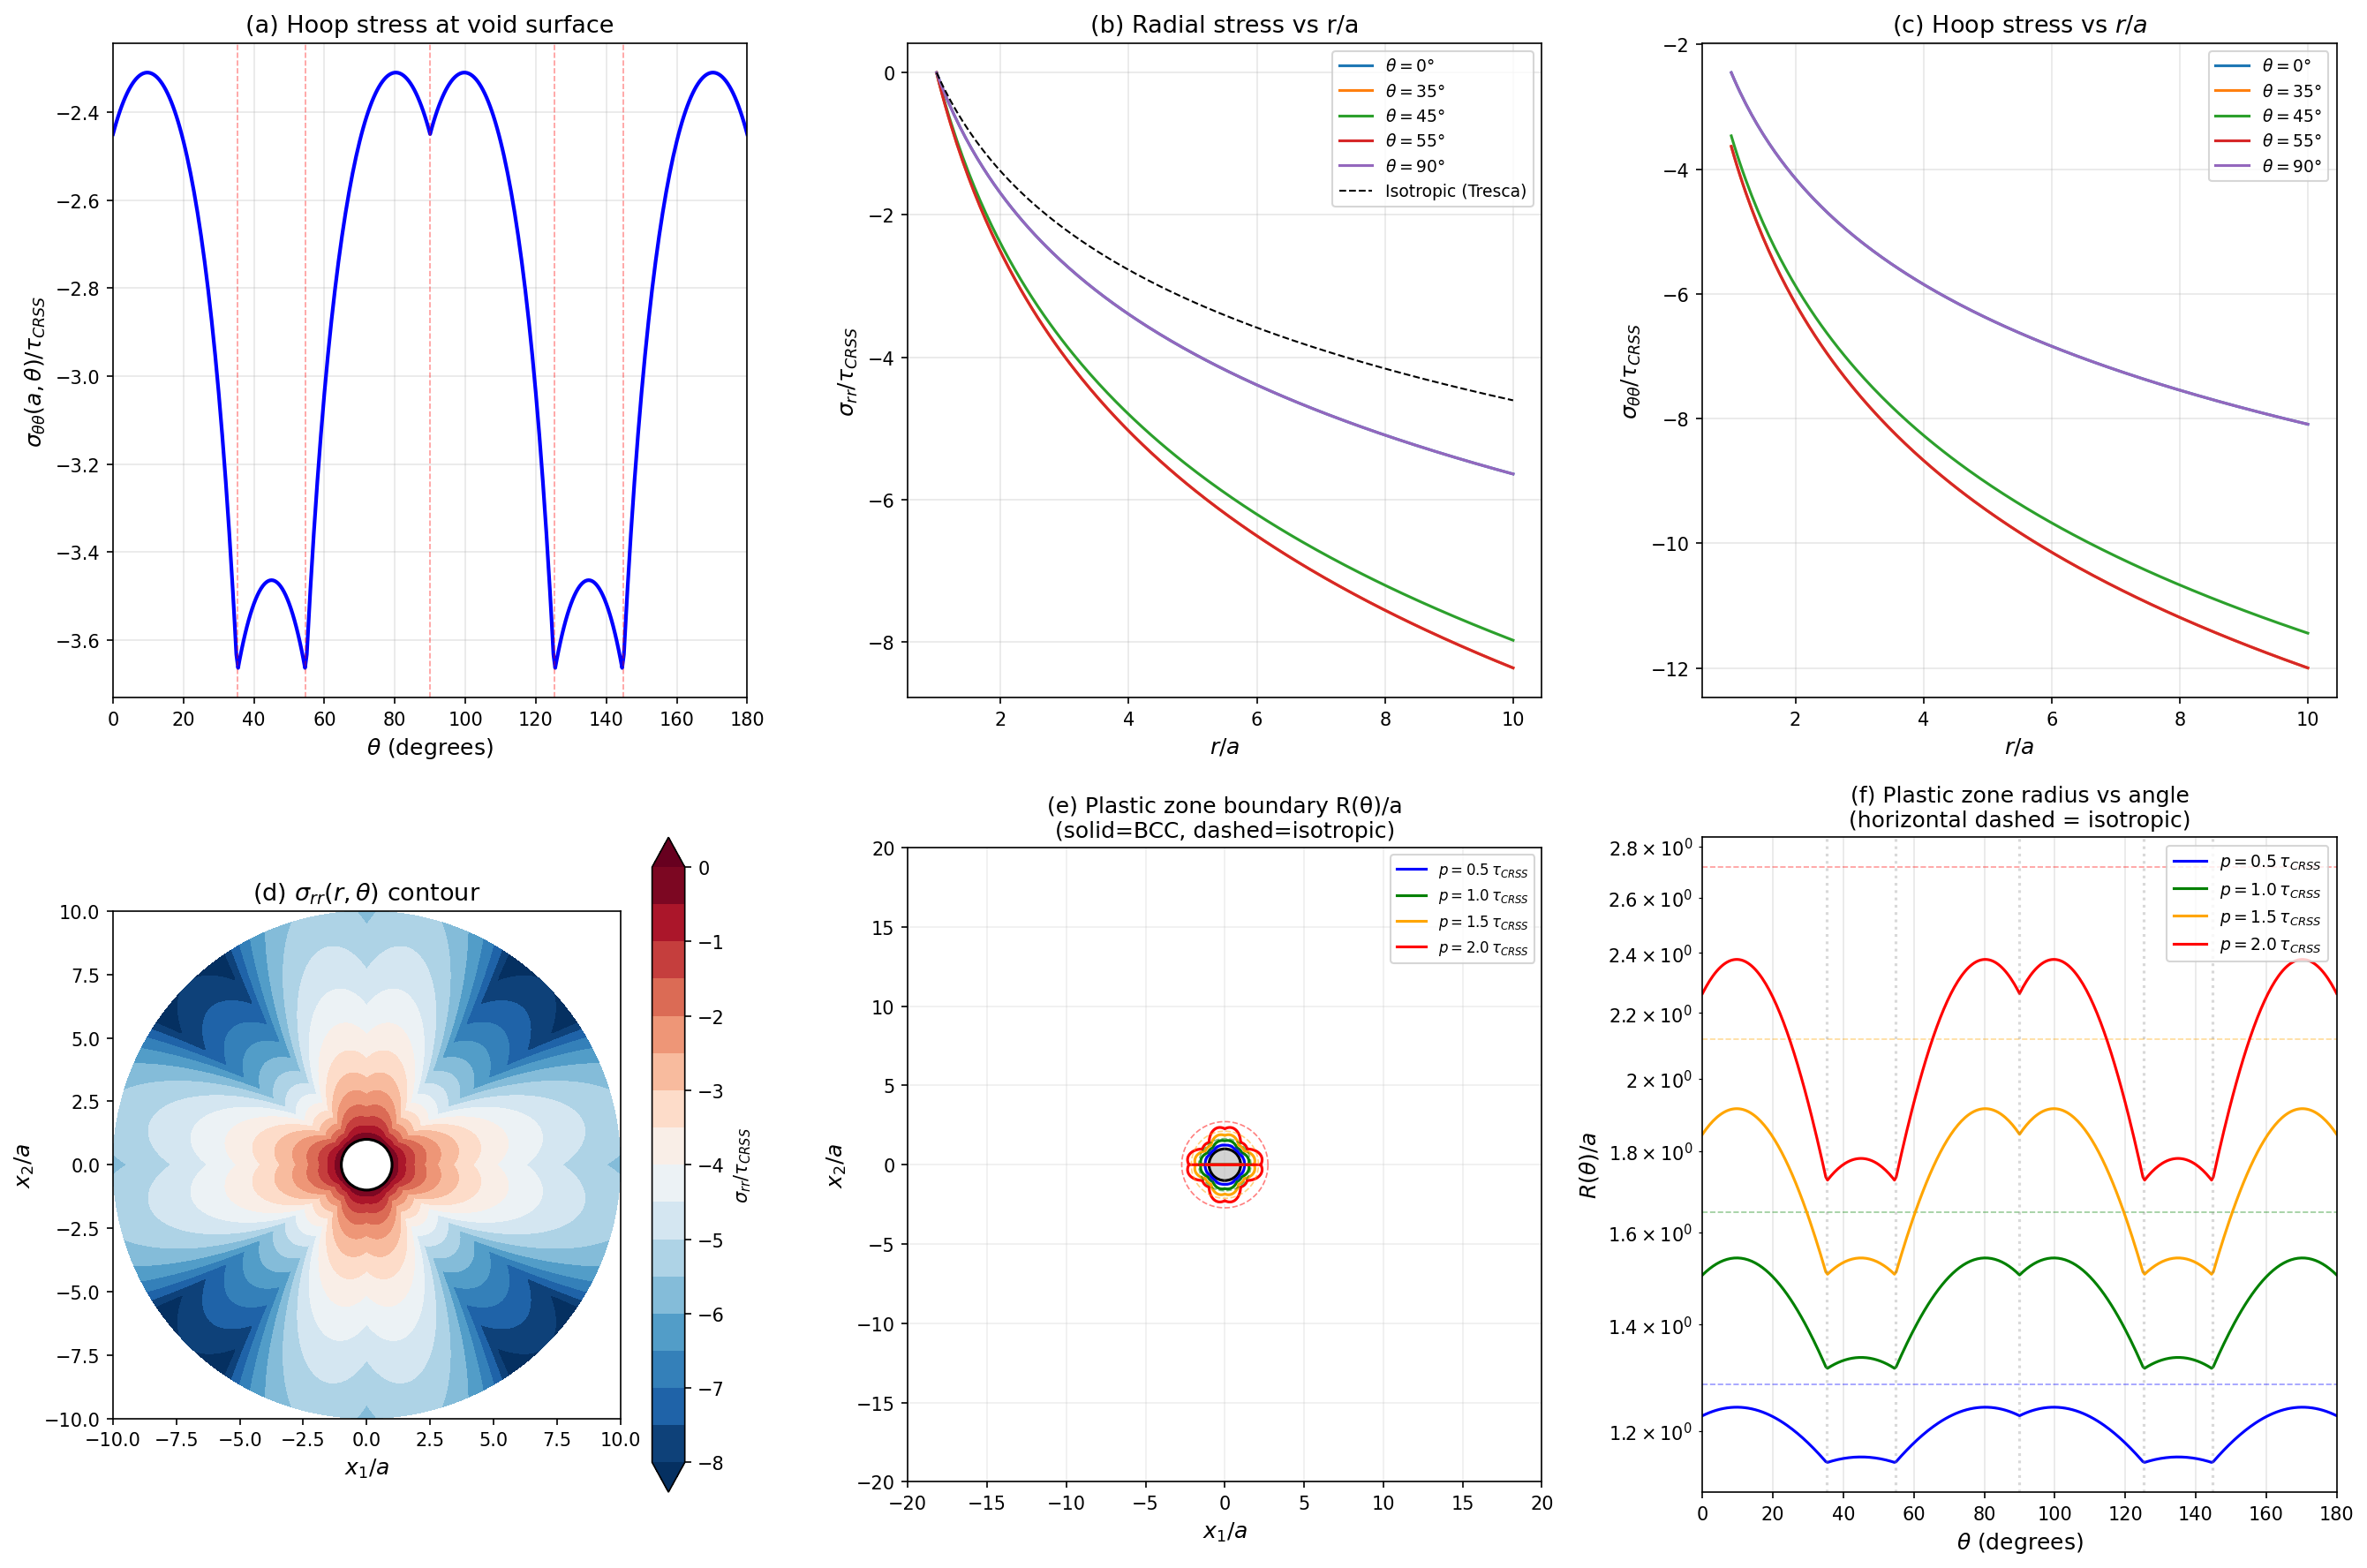
\includegraphics[width=0.95\textwidth]{../figures/interior_stress_field}
\caption{Interior stress field. (a)~Hoop stress at void surface.
(b,c)~Radial and hoop stress versus $r/a$.
(d)~Contour plot of $\srr(r, \theta)$.
(e)~Non-circular plastic zone boundary (solid = BCC, dashed = isotropic).
(f)~Plastic zone radius versus angle.}
\label{fig:interior}
\end{figure}

% ============================================================
\section{Activation pressure}
\label{sec:activation}
% ============================================================

The activation pressure $p^*$ is the far-field equibiaxial stress required
to sustain full plastic flow around the void. It is determined by the
maximum $|\sm|$ at the void surface, which occurs at the sector boundaries
$\theta = \theta_1$ and $\theta = \theta_2$:
\begin{equation}
\label{eq:activation}
\boxed{p^* = \frac{3\sqrt{6}}{4}\,\tcrss \approx 1.837\,\tcrss.}
\end{equation}

Table~\ref{tab:activation} compares this result with isotropic and FCC
values.

\begin{table}[htb]
\caption{Activation pressure for void growth in different materials.}
\label{tab:activation}
\centering
\begin{tabular}{lcc}
\toprule
Material & $p^* / \tcrss$ & Ratio to isotropic \\
\midrule
Isotropic (Tresca)            & $1.000$ & $1.00$ \\
Isotropic (von Mises)         & $2/\sqrt{3} \approx 1.155$ & $1.15$ \\
FCC $\{111\}\langle 110\rangle$ (Kysar, 2005) & $\sqrt{6}/2 \approx 1.225$ & $1.22$ \\
\textbf{BCC} $\{110\}\langle 111\rangle$ \textbf{(this work)}
                              & $3\sqrt{6}/4 \approx 1.837$ & $1.84$ \\
\bottomrule
\end{tabular}
\end{table}

The BCC activation pressure exceeds the FCC value by a factor of
\begin{equation}
\label{eq:ratio}
\frac{p^*_{\mathrm{BCC}}}{p^*_{\mathrm{FCC}}}
  = \frac{3\sqrt{6}/4}{\sqrt{6}/2} = \frac{3}{2},
\end{equation}
which is \emph{exactly} $3/2$, independent of material parameters.

% ============================================================
\section{Comparison of BCC and FCC solutions}
\label{sec:comparison}
% ============================================================

% TODO: Reproduce FCC solution in the same framework for side-by-side
% comparison. Include:
% - Yield polygon overlay
% - Sector boundary comparison
% - Stress field comparison
% - Velocity field comparison

\begin{table}[htb]
\caption{Comparison of BCC and FCC void solutions.}
\label{tab:comparison}
\centering
\begin{tabular}{lcc}
\toprule
Property & FCC $\{111\}\langle 110\rangle$ & BCC $\{110\}\langle 111\rangle$ \\
\midrule
Effective in-plane constraints & 3 & 3 \\
Yield polygon shape  & Regular hexagon & Elongated hexagon \\
Max $|X|$ (half-width) & $\sqrt{6}/2$ & $\sqrt{6}/2$ \\
Max $|Y|$ (half-height) & $1$ & $\sqrt{3}$ \\
Aspect ratio & $\sqrt{2/3} \approx 0.82$ & $\sqrt{8/3} \approx 1.63$ \\
Sectors in $[0,\pi]$ & 6 & 6 \\
Key angle & $\arctan\sqrt{2}$ & $\arctan(2\sqrt{2})$ \\
Activation pressure $p^*$ & $\sqrt{6}/2\;\tcrss$ & $3\sqrt{6}/4\;\tcrss$ \\
Anti-plane-only systems & 0 & 2 (systems 1, 2) \\
Cross-plane pairings & 0 of 3 & 2 of 3 \\
Plastic zone shape & Non-circular & Non-circular (4-lobed) \\
\bottomrule
\end{tabular}
\end{table}

% ============================================================
\section{Numerical verification}
\label{sec:numerical}
% ============================================================

% TODO: Crystal plasticity FEM verification
% - Model setup: cylindrical void, BCC {110}<111>, equibiaxial loading
% - Compare: void surface stress, sector boundaries, activation pressure
% - Also possible: atlas-PINN verification using existing framework

% ============================================================
\section{Discussion}
\label{sec:discussion}
% ============================================================

\subsection{Radiation void swelling resistance}

The result $p^*_{\mathrm{BCC}} / p^*_{\mathrm{FCC}} = 3/2$ provides a
quantitative, single-crystal-level explanation for the superior resistance
of BCC metals to radiation-induced void swelling. The 50\% higher
activation pressure means that, for a given irradiation-induced stress
state, BCC crystals require significantly more driving force to grow voids
plastically. This complements existing explanations based on vacancy
mobility and dislocation bias~\citep{zinkle2013}.

\subsection{Anti-plane shear systems}

The finding that systems 1 and 2 have identically zero in-plane Schmid
factor has implications beyond the void problem. In any plane strain
problem on the $(110)$ plane, these two systems (on the $(110)$ slip plane
itself) can only contribute anti-plane shear --- they cannot accommodate
any in-plane plastic strain. This reduces the effective number of
in-plane slip systems from 12 to 10.

\subsection{Non-circular plastic zone}

The predicted four-lobed plastic zone shape
(Fig.~\ref{fig:interior}e) is a direct consequence of the crystal
anisotropy and represents a qualitative difference from isotropic
solutions. This shape will affect void-void interactions in polycrystalline
materials: the plastic zones of adjacent voids will overlap at
orientation-dependent distances, making void coalescence a function of
crystal orientation.

\subsection{Implications for ductile fracture models}

% TODO: Discuss implications for:
% - Crystal plasticity damage models (Keralavarma-Benzerga type)
% - Orientation-dependent void growth rates
% - Homogenized Gurson-type models for BCC polycrystals

% ============================================================
\section{Conclusions}
\label{sec:conclusions}
% ============================================================

The analytical stress field around a cylindrical void in a rigid-ideally
plastic BCC $\{110\}\langle 111\rangle$ single crystal has been derived
using Rice's anisotropic slip line theory. The principal findings are:

\begin{enumerate}
\item The twelve BCC slip systems reduce to three distinct in-plane yield
constraints under plane strain with void axis $\|[110]$. Systems 1 and 2
(on the $(110)$ plane containing the void axis) have zero in-plane Schmid
factor.

\item The yield polygon in the Mohr stress plane is a hexagon with vertices
at $(\pm\sqrt{6}/2, 0)$ and $(\pm\sqrt{6}/4, \pm\sqrt{3})$, elongated
in the shear direction with aspect ratio $\sqrt{8/3} \approx 1.63$.

\item The stress field decomposes into six angular sectors in $[0, \pi]$
with exact boundaries at $\theta_1 = \frac{1}{2}\arctan(2\sqrt{2})
\approx 35.3^\circ$ and $\theta_2 = \frac{1}{2}[\pi - \arctan(2\sqrt{2})]
\approx 54.7^\circ$.

\item The activation pressure is
$p^* = \frac{3\sqrt{6}}{4}\,\tcrss \approx 1.84\,\tcrss$, which is
exactly $3/2$ times the FCC value. This provides a quantitative
explanation for the superior radiation void swelling resistance of BCC
metals.

\item The plastic zone surrounding the void is non-circular, with a
four-lobed shape reflecting the crystal symmetry of the $(110)$ plane.
\end{enumerate}

\begin{acknowledgements}
% TODO: Acknowledgements
\end{acknowledgements}

% ============================================================
\bibliographystyle{plainnat}
\bibliography{references}

\end{document}
